\documentclass[a4paper]{article}

\usepackage[english]{babel}
\usepackage[utf8]{inputenc}
\usepackage{fullpage}
\usepackage{amsmath}
\usepackage{graphicx}
\usepackage[colorinlistoftodos]{todonotes}
\usepackage{hyperref}
\usepackage{amssymb}
\usepackage{outline} \usepackage{pmgraph} \usepackage[normalem]{ulem}
\usepackage{graphicx} \usepackage{verbatim}
% \usepackage{minted} % need `-shell-escape' argument for local compile

\usepackage[UTF8]{ctex}
\usepackage[inkscapeformat=png]{svg}

\title{
    \vspace*{1.5in}
    \includesvg[width=2.75in]{figures/logo.svg} \\
    \vspace*{1in}
    \textbf{\huge Biweekly Report}
    \vspace{0.5in}
}

\author{ \\
    \textbf{userElaina} \\
    \vspace*{1in}
}

\date{八月上}
\setcounter{page}{-1}
\newpage

\begin{document}

\maketitle
\tableofcontents
% \setcounter{page}{0}
\thispagestyle{empty}
\newpage


\section{了解 SNN}

\subsection{神经元模型}

\begin{figure}[hb]
    \centering
    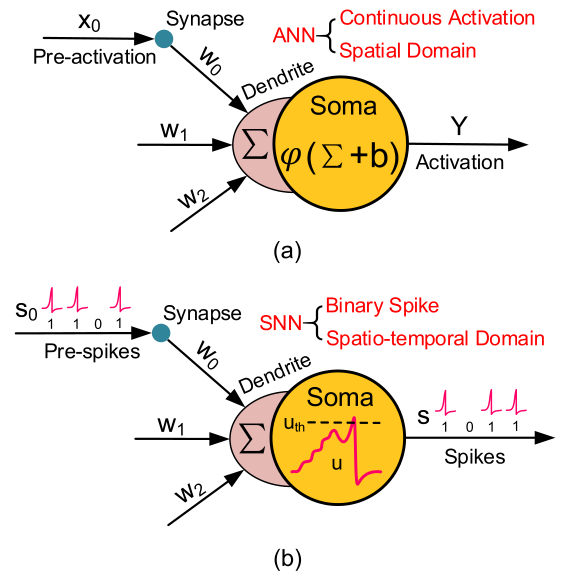
\includegraphics[width=0.8\textwidth]{figures/s1.png}
    \caption{ANN 和 SNN 的基本神经元}
    \label{fig:s1}
\end{figure}

\begin{itemize}
    \item\begin{equation*}
        \begin{aligned}
            \tau\frac{{\rm d}V(t)}{{\rm d}t} &= X(t) \\
            V_t &= V_{t-1}+\frac{1}{\tau}X_t
        \end{aligned}
    \end{equation*}
    \item\begin{equation*}
        \begin{aligned}
            \tau\frac{{\rm d}V(t)}{{\rm d}t} &= -V(t)+X(t) \\
            V_t &= (1-\frac{1}{\tau})V_{t-1}+\frac{1}{\tau} X_t
        \end{aligned}
    \end{equation*}
\end{itemize}

\subsection{结构}

类似 ANN, 事件驱动.

\subsection{编码}

Rate coding, temporal coding 等.

\section{阅读文献}

\begin{itemize}
    \item \href{http://proceedings.mlr.press/v139/li21d/li21d.pdf}{A Free Lunch From ANN: Towards Efficient, Accurate Spiking Neural Networks Calibration}
    \item \href{https://www.frontiersin.org/articles/10.3389/fnins.2016.00508/full}{Training deep spiking neural networks using backpropagation}
    \item \href{https://www.frontiersin.org/articles/10.3389/fnins.2018.00331/full}{Spatio-temporal backpropagation for training high-performance spiking neural networks}
    \item \href{https://openaccess.thecvf.com/content/CVPR2022/papers/Meng_Training_High-Performance_Low-Latency_Spiking_Neural_Networks_by_Differentiation_on_Spike_CVPR_2022_paper.pdf}{Training High-Performance Low-Latency Spiking Neural Networks by Differentiation on Spike Representation}
\end{itemize}

\section{看讲座}

视觉与学习青年学者研讨会.

\section{其它}

双周报 LaTeX 模板, 周报 PPT LaTeX 模板.

\end{document}
